%%%%%% Configurando os pacotes e comandos %%%%%%
%%%%%% Pule para a linha 62 %%%%%%%
\documentclass[fontsize=11pt]{article}
\usepackage[margin=0.70in]{geometry}
\usepackage{lipsum,mwe,abstract}
\usepackage[T1]{fontenc} 
\usepackage[brazilian]{babel} 
\usepackage{setspace}
\usepackage{caption}
\usepackage[hidelinks]{hyperref}
\usepackage{multirow}

\usepackage{fancyhdr} % Custom headers and footers
%\pagestyle{fancyplain} % Makes all pages in the document conform to the custom headers and footers
%\fancyhead{} 
%\fancyfoot[C]{\thepage} % Page numbering for right footer
\setlength\parindent{0pt} 
\setstretch{1.5}

\usepackage{amsmath,amsfonts,amsthm, amssymb} % Math packages
\usepackage{wrapfig}
\usepackage{graphicx}
\usepackage{float}
\usepackage{subcaption}
\usepackage{comment}
\usepackage{enumitem}
\usepackage{cuted}
\usepackage{sectsty} % Allows customizing section commands
% \allsectionsfont{\normalfont \large \scshape} % Section names in small caps and normal fonts
\usepackage{biblatex}
\addbibresource{references.bib}

%code things
\usepackage{xcolor}
\usepackage{listings}

\lstdefinestyle{customc}{
  belowcaptionskip=1\baselineskip,
  breaklines=true,
  frame=L,
  xleftmargin=\parindent,
  language=C,
  showstringspaces=false,
  basicstyle=\small\ttfamily,
  keywordstyle=\bfseries\color{green!40!black},
  commentstyle=\itshape\color{purple!40!black},
  identifierstyle=\color{blue},
  stringstyle=\color{orange},
}
%%%

\definecolor{codegreen}{rgb}{0,0.6,0}
\definecolor{codegray}{rgb}{0.5,0.5,0.5}
\definecolor{codepurple}{rgb}{0.58,0,0.82}
\definecolor{backcolour}{rgb}{0.95,0.95,0.92}

\lstdefinestyle{mystyle}{
  backgroundcolor=\color{white},   
  commentstyle=\color{codegreen},
  keywordstyle=\color{magenta},
  numberstyle=\tiny\color{codegray},
  stringstyle=\color{codepurple},
  basicstyle=\linespread{0.9}\ttfamily\footnotesize,
  breakatwhitespace=false,         
  breaklines=true,                 
  captionpos=b,                    
  keepspaces=true,                 
  numbers=left,                    
  numbersep=5pt,                  
  showspaces=false,                
  showstringspaces=false,
  showtabs=false,                  
  tabsize=2,
  language=C
}
\lstset{escapechar=@,style=mystyle}
  
  
  \renewenvironment{abstract} % Change how the abstract look to remove margins
  {\small
  \begin{center}
  \bfseries \abstractname\vspace{-.5em}\vspace{0pt}
  \end{center}
  \list{}{%
    \setlength{\leftmargin}{0mm}
    \setlength{\rightmargin}{\leftmargin}%
  }
  \item\relax}
 {\endlist}
 
\makeatletter
\renewcommand{\maketitle}{\bgroup\setlength{\parindent}{0pt}% Change how the title looks like
\begin{center}
    \textbf{
      Universidade de São Paulo\\
      Instituto de Ciências Matemáticas e Computação
    }
\end{center}
\begin{flushleft}
  \textbf{\@title}
  \@author\\
  [3pt] 
  \@date
\end{flushleft}\egroup
}
\makeatother
%%% Daqui pra cima é apenas configuração %%%
%%%%%%%%%%%%%%%%%%%%%%%%%%%%%%%%%%%%%%%%%%%%

%%%%%% Definindo seus dados %%%%%%
\title{
\Large{Relatório 3 de Laboratório de Introdução à Ciências da Computação 2}\\
[10pt] 
}
\author{Vítor Amorim Fróis} 
\date{\today}
%%%%%%%%%%%%%%%%%%%%%%%%%%%%%%%%%%%

%%%%%% Iniciando seu relatório %%%%%% 
\begin{document}
\maketitle

\begin{abstract}
  %%%%%% Contextualize o seu trabalho. %%%%%%%
  No módulo 2 da disciplina de LICC2 buscamos analisar métodos de ordenação mais complexos que os tradicionais Bubble, Insertion e Merge, que podem ter complexidade de até $O(n^2)$. Aqui, Heap e Quick buscam o limite inferior de $O(n\log n)$. Na parte de metodologia são feitos os cálculos para provar esse valor enquanto na parte de resultados é possível comparar o que foi feito aqui com outros métodos e confirmar que a complexidade perfoma como esperado.
\end{abstract}

\rule{\linewidth}{0.2pt}

\section{Introdução}
    %%%%%% Faça a introdução do seu relatório. O que será feito? %%%%%%
    Durante o módulo 1, métodos de ordenação simples, como o Bubble, Insertion
    e Merge. Os dois primeiros tinham complexidade $O(n^2)$, enquanto o Merge 
    conseguia alcançar complexidade linear-logarítmica.
    Agora, através de novas ideias, é preciso aprimorar os métodos para buscar
    complexidade $O(n\log n)$ corriqueiramente. Esses são Heap e Quick. 

\section{Metodologia e desenvolvimento}
  \subsection{Heap Sort}
    O Heap Sort é um método de ordenação que usa a estrutura chamada de Heap.
    Essa é uma estrutura semelhante a uma árvore binária, mas também pode ser 
    representada através de um vetor. 
    \\ No algoritmo, os elementos são posicionados em max heap, operação que possui 
    complexidade $O(\log n)$ \cite{heapSort}. 
    \lstinputlisting[linerange={39-55}]{sorts.c}
    Então, troca os elementos $[1];[n]$ de posição e descarta
    o último elemento ao diminuir o tamanho $n$ do vetor \cite{mitvideo}. 
    \lstinputlisting[linerange={60-63}]{sorts.c}
    Novas chamadas 
    recursivas são executadas até que o vetor esteja completamente ordenado.
    Como é necessário passar pelo vetor uma vez para executar esse método,
    a complexidade é $O(n) \times O(\log n) = O(n\log n)$.
    Já que independente dos casos o mesmo algoritmo sempre é executado, 
    o pior caso é igual ao maior caso.
    A complexidade de espaço é $O(1)$, usada apenas para os \textit{swaps}.

  \subsection{Quick Sort}
    Já o Quick Sort é um algoritmo de ordenação muito eficiente que utiliza pivôs para ordenação. 
    A partir desse elemento, chamadas recursivas onde cada elemento deve ser menor que o pivô 
    são feitas e a ordenação se completa.
    Para o algoritmo manter sua alta eficiência, é necessário que a escolha de pivô seja bem 
    feita. Assim, uma técnica utilizada é fazer a mediana entre o primeiro, último e elemento médio
    do vetor. Isso busca garantir que o elemento escolhido esteja o mais próximo da média de valores 
    sem muito poder computacional.
    \lstinputlisting[linerange={82-91}]{sorts.c}
    No pior caso, as chamadas recursivas são do tipo $n-1$, e assim o algoritmo deve percorrer
    todo o vetor, elemento a elemento, para ordenar.
    Contudo, no melhor caso possível, há chamadas recursivas de tamanho $\dfrac{n}{2} - 1$ 
    (considere $n$ o tamanho da chamada recursiva anterior), de forma
    que o melhor caso executa $\log_2 n$ chamadas \cite{moacir}.
    \lstinputlisting[linerange={92-127}]{sorts.c}
    Pela análise do algoritmo, cada chamada possui complexidade $O(n)$. Assim, no melhor caso, 
    o algoritmo faz $\log n$ chamadas de $O(n)$, resultando em complexidade de tempo $O(n\log n)$.
    Um ponto importante de se destacar é a não utilização de vetores auxiliares, que 
    traz complexidade de espaço 0 para o algoritmo.
  \subsection{Comparação com métodos do módulo 1}  
    Apesar de compartilharem complexidade com Merge, os métodos estudados 
    no módulo presente são melhores que Insertion e Bubble. Assim, no caso médio,
    espera-se que log-lineares se sobressaiam, enquanto aqueles de ordem 
    quadrática performem pior. Ainda assim, cada método, mesmo que com piores
    constantes, pode ser útil em ocasiões especiais.
\section{Resultados}
  %%%%%% Mostre os resultados obtidos através dos cálculos. Utilize imagens se necessário. %%%%%%
  Para comparar Heap e Quick, serão plotados inicialmente gráficos até 10k e 100k.
  Então, um gráfico especial para o Quick será produzido a fim de aprofundar
  no pior caso desse algoritmo, que segundo a parte de Metodologia, tem 
  complexidade $O(n^2)$.
  \subsection{Caso Médio}
    É esperado que ao \textit{plottar} os gráficos
    das funções, os comportamentos sejam parecidos, já que a complexidade é igual,
    ao menos no caso médio.
    \begin{figure}[H]
      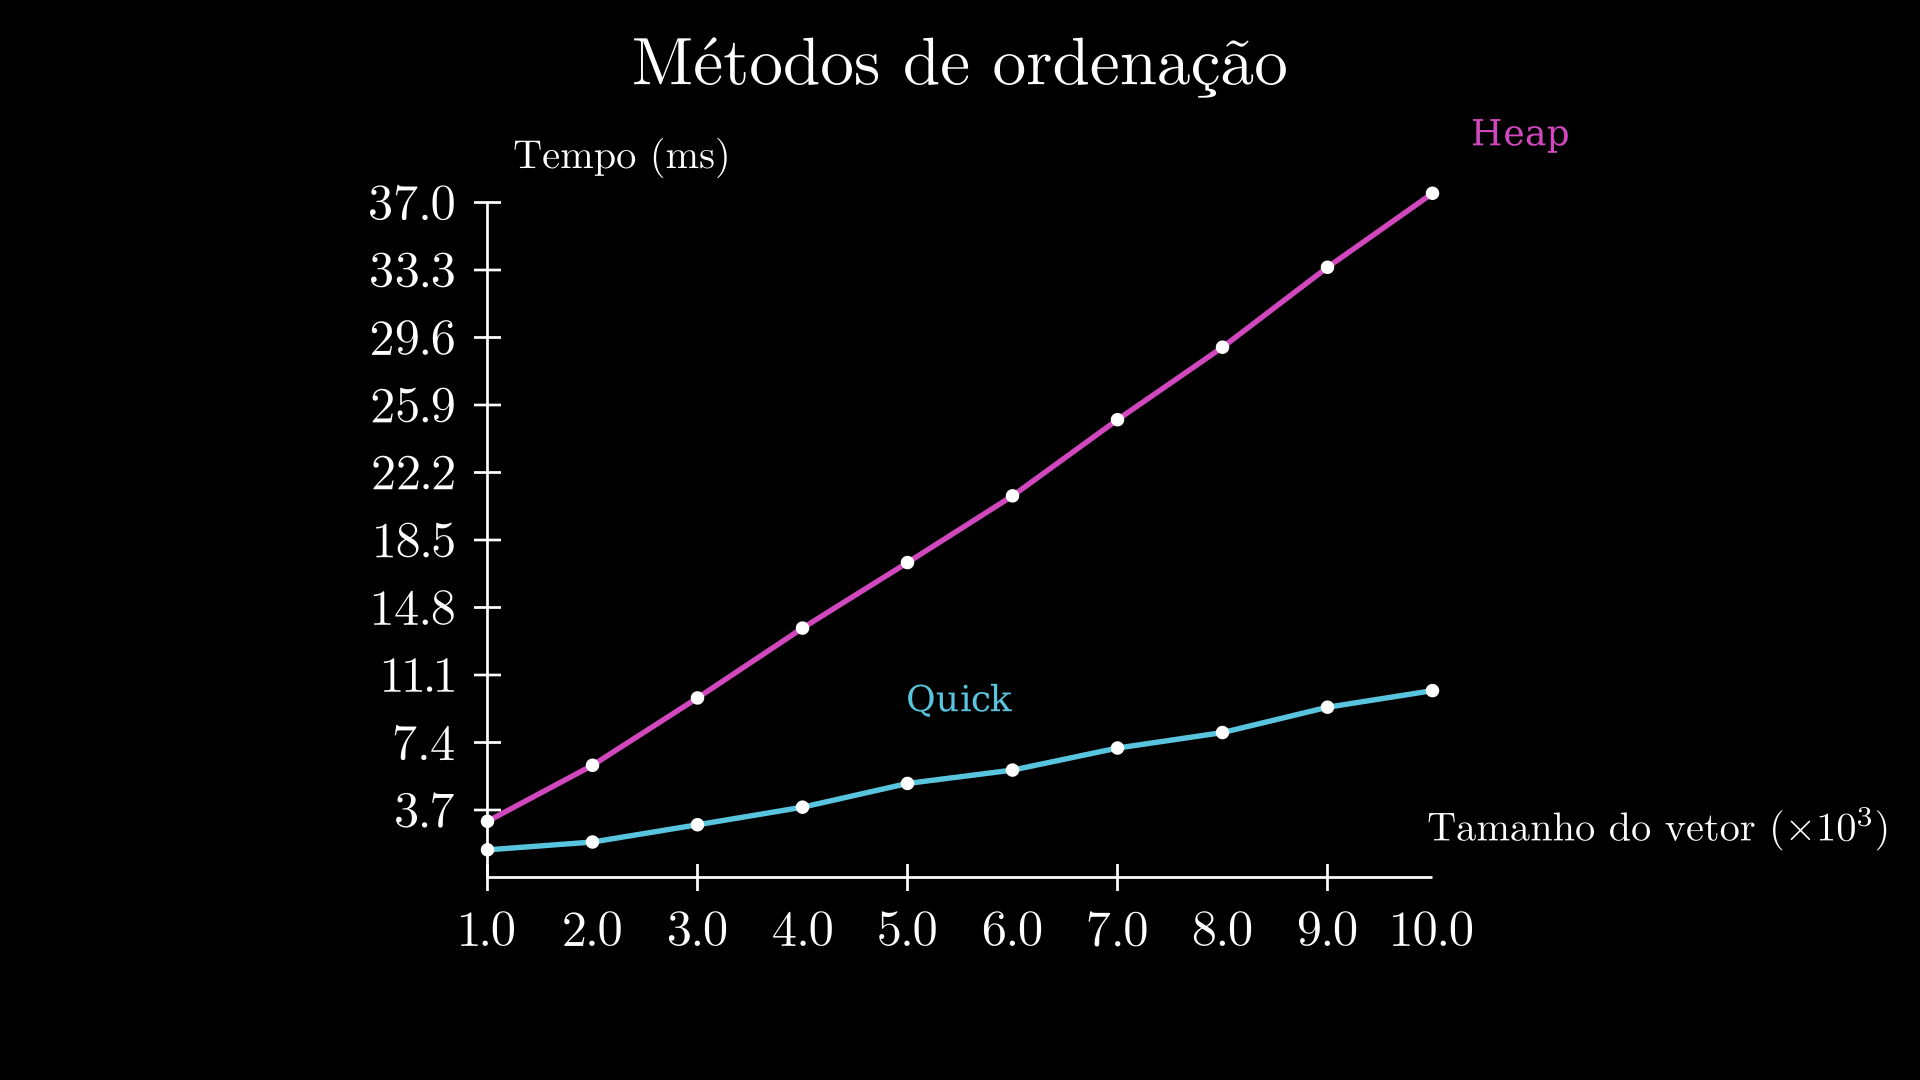
\includegraphics[width=\textwidth]{graph10k.png} 
      \caption{Ordenação de vetores randômicos com até 10000 elementos}
      \label{fig:10k}
    \end{figure}
    A primeira coisa que chama atenção nesse gráfico é a disparidade entre o Heap
    e o Quick. Isso se deve ao fato de que as constantes do primeiro são muito 
    maiores que as do segundo. Ainda é possível notar que apesar de parecer uma reta, 
    o gráfico possui uma leve inclinação, originária do $\log_2 n$ na função de 
    complexidade.
    \\ Com o tempo, a função logarítimica tende a encontrar uma inclinação menor, 
    portanto quanto maior o valor de $n$, mais $O(n \log_2 n)$ se aproxima, proporcionalmente,
    de uma função linear. Observar o gráfico com valores até 100000 
    permite melhor visualização.
    \begin{figure}[H]
      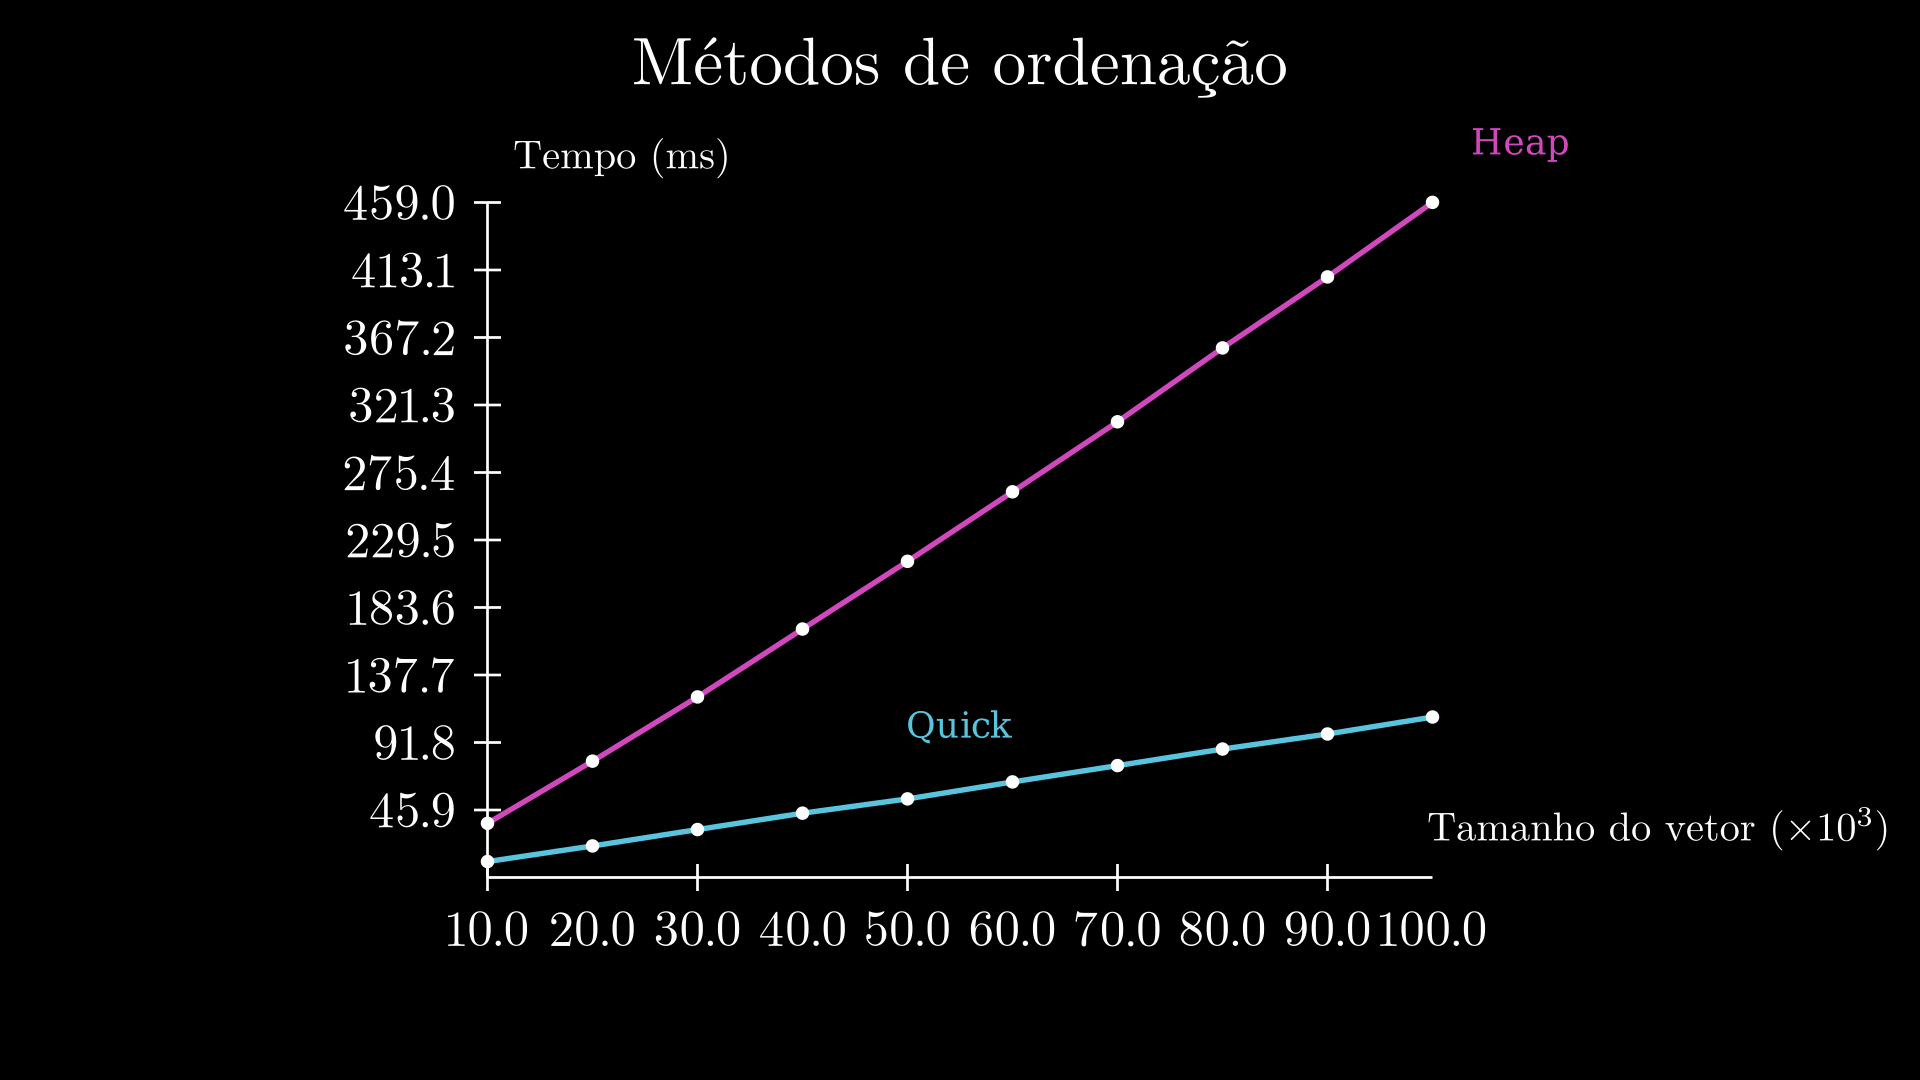
\includegraphics[width=\textwidth]{graph100k.png} 
      \caption{Ordenação de vetores randômicos com até 100000 elementos}
      \label{fig:100k}
    \end{figure}
  \subsection{Pior Caso}
    Entre os dois algoritmos estudados, somente o Quick apresenta pior
    caso. Assim, o gráfico busca comparar seu pior caso com o caso médio
    do Heap.
    \lstinputlisting[linerange={130-131}]{sorts.c}
    O pivo será escolhido como o primeiro elemento do vetor, o qual estará
    inversamente ordenado.
    \begin{figure}[H]
      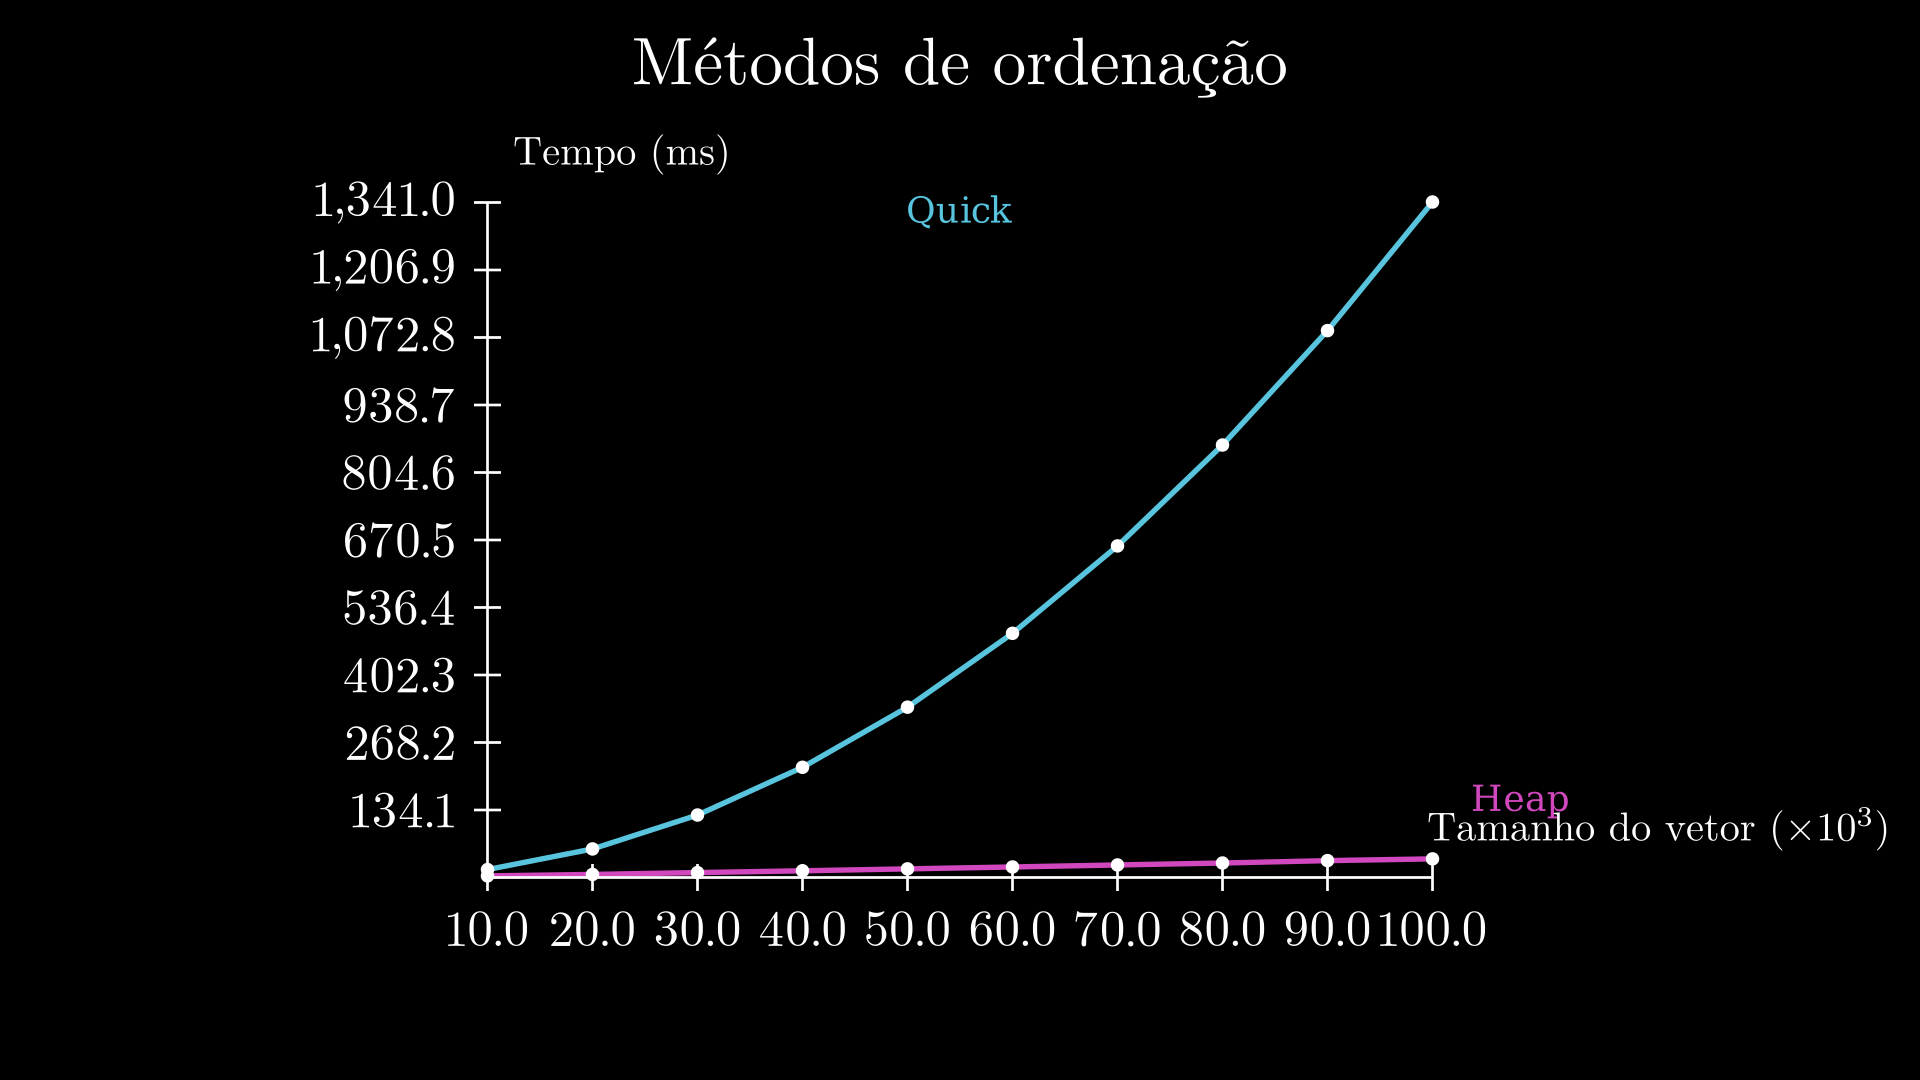
\includegraphics[width=\textwidth]{quickWorse.png} 
      \caption{Pior caso do Quick Sort}
      \label{fig:worse}
    \end{figure}
    Assim, pode se observar que em seu pior caso, o Quick Sort realmente  apresenta complexidade $O(n^2)$, enquanto o Heap continua com pior caso
    $O(n \log n)$.
  \subsection{Comparação com métodos anteriores}
    Ao comparar com os métodos anteriores, o gráfico do caso médio se porta como esperado
    Nota-se que o Insertion dispara, enquanto os métodos que possuem complexidade $O(n\log n)$
    ficam próximos. A pequena diferença entre eles se dá pelas constantes, como já comentado
    anteriormente.
    \begin{figure}[H]
      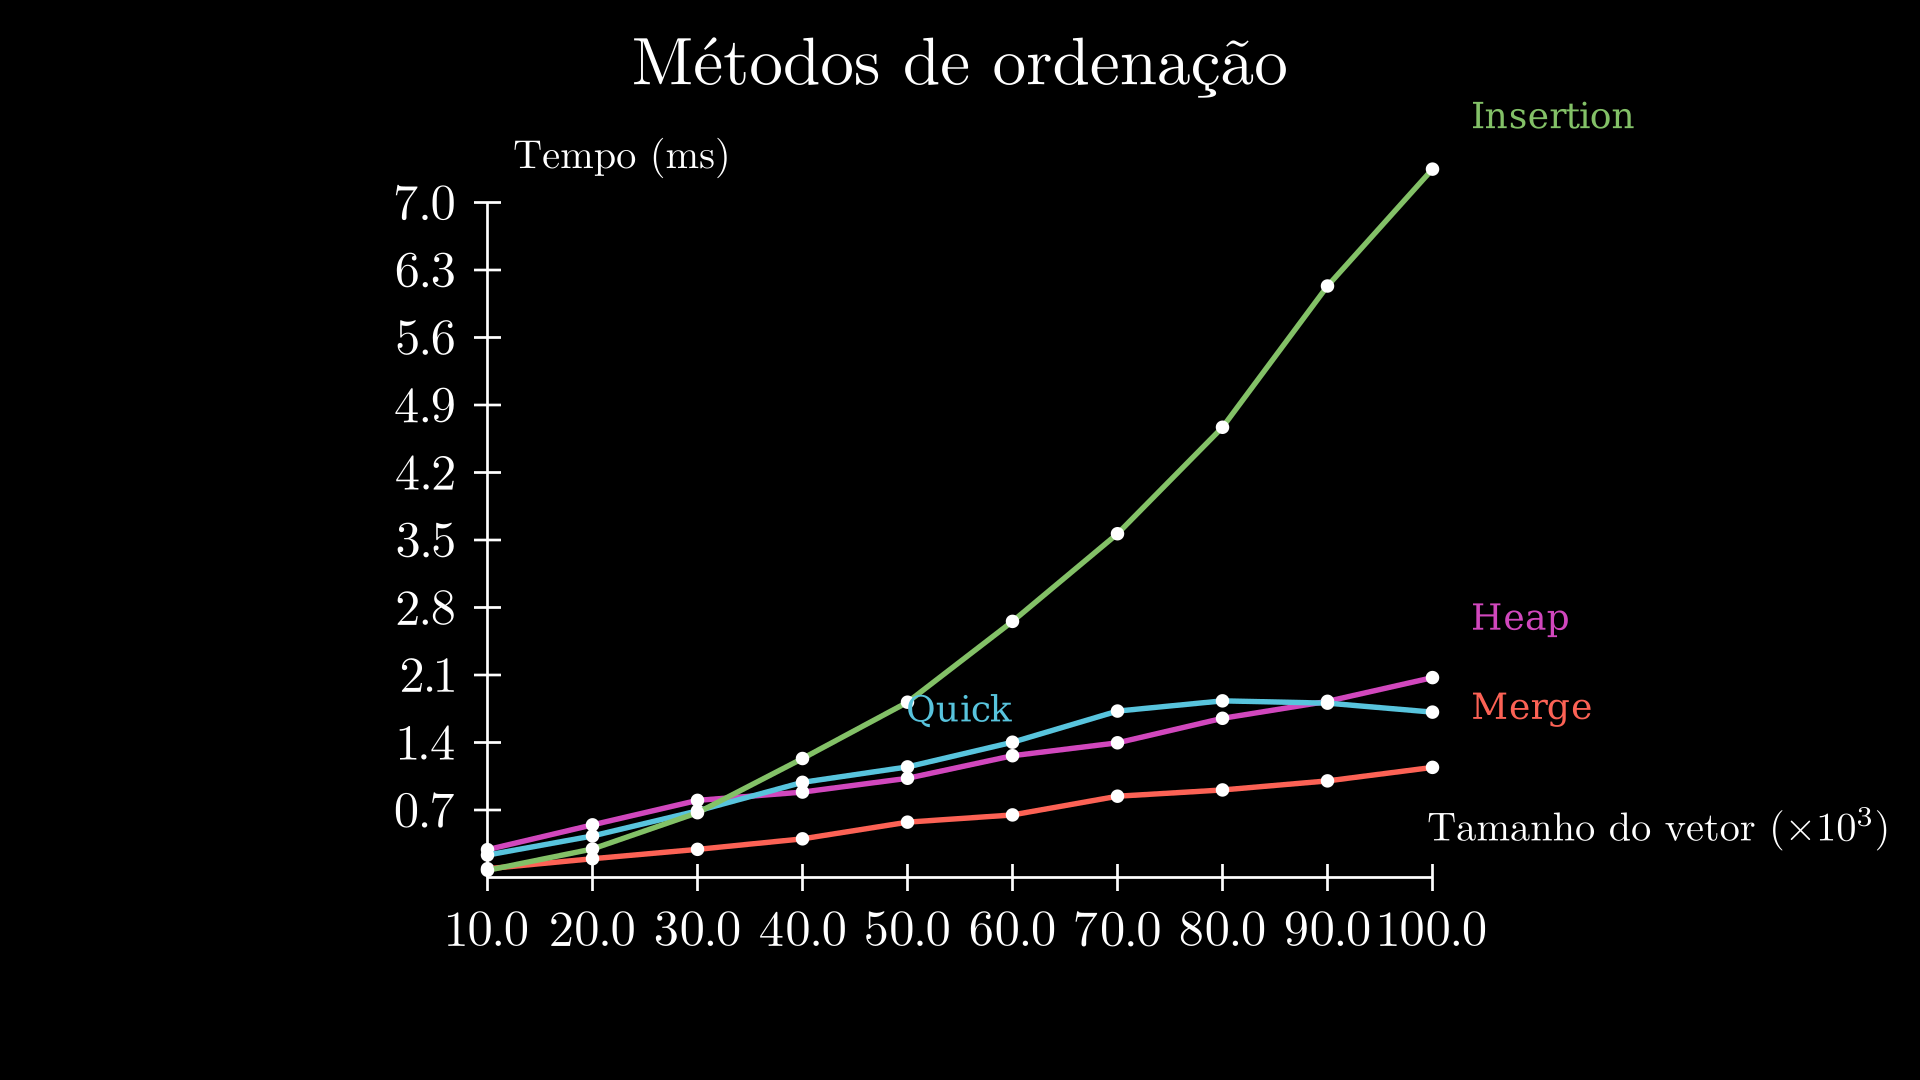
\includegraphics[width=\textwidth]{allgraphs.png} 
      \caption{Todos métodos de ordenação}
      \label{fig:all}
    \end{figure}

  \section{Conclusão}
  %%%%%% Conclusão do relatório. O que você aprendeu nessa tarefa? %%%%%%
  Concluímos ao longo do relatório que os dois algoritmos são muito eficientes,
  porém, o Heap é tem uma garantia maior de complexidade baixa. Para usar o Quick Sort,
  é essencial garantir que o pivô escolhido seja bom, caso contrário sua 
  complexidade dispara, tornando-se $O(n^2)$.
  \\ É também possível observar que as análises feitas na seção de Metodologias 
  tiveram seus resultados confirmados, sendo mais fácil constatar ao comparar
  os algoritmos do segundo módulo com os do primeiro.
  \\ Ainda assim, cada método possui sua particularidade, e analisar um problema
  e suas nuances antes de escolher um algoritmo para resolver é essencial.
\printbibliography[heading=bibintoc, title={Referências}]
    %%%%%% Lembre-se de adicionar as referências bibliográficas utilizadas no arquivo 'references.bib'e depois cita-las nessa seção. Conulta: https://pt.overleaf.com/learn/latex/Bibliography_management_in_LaTeX %%%%%%

\end{document}

 